
\documentclass{beamer}
\DeclareGraphicsExtensions{.jpg, .pdf,.png,.eps}
\setbeamertemplate{caption}{\raggedright\insertcaption\par}

\usepackage{graphicx}
\title{MC-Cons 2.0}
\author{Gabriel Parent}



\usetheme{Execushares}

\begin{document}

\maketitle


\section{introduction}

\begin{frame}
	\frametitle{I work with 2D structures}
	\begin{figure}[!htb]
	\centering
	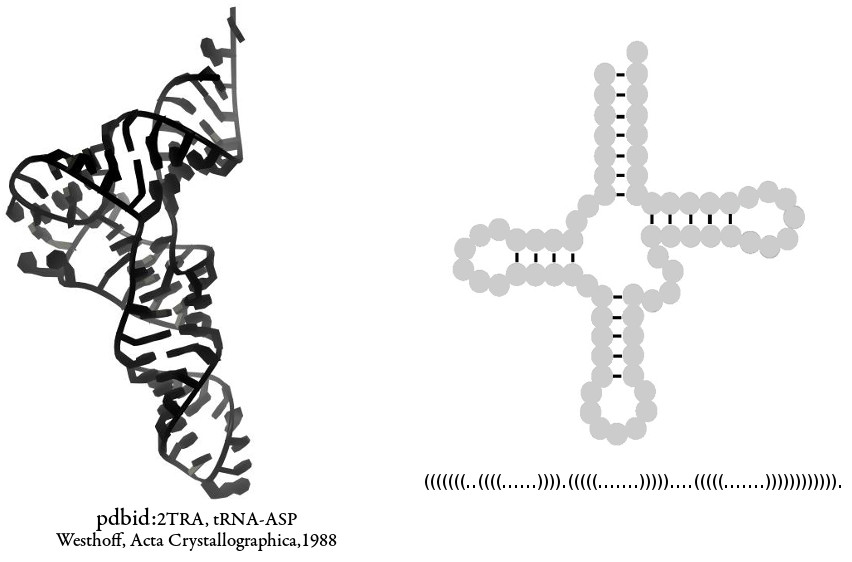
\includegraphics[scale=0.39]{figs/representations}
	%\caption{there are lots of ways to represent structure}
	\end{figure} 
\end{frame}


\begin{frame}
	\frametitle{one RNA has many structures}
	\begin{figure}
	\centering
	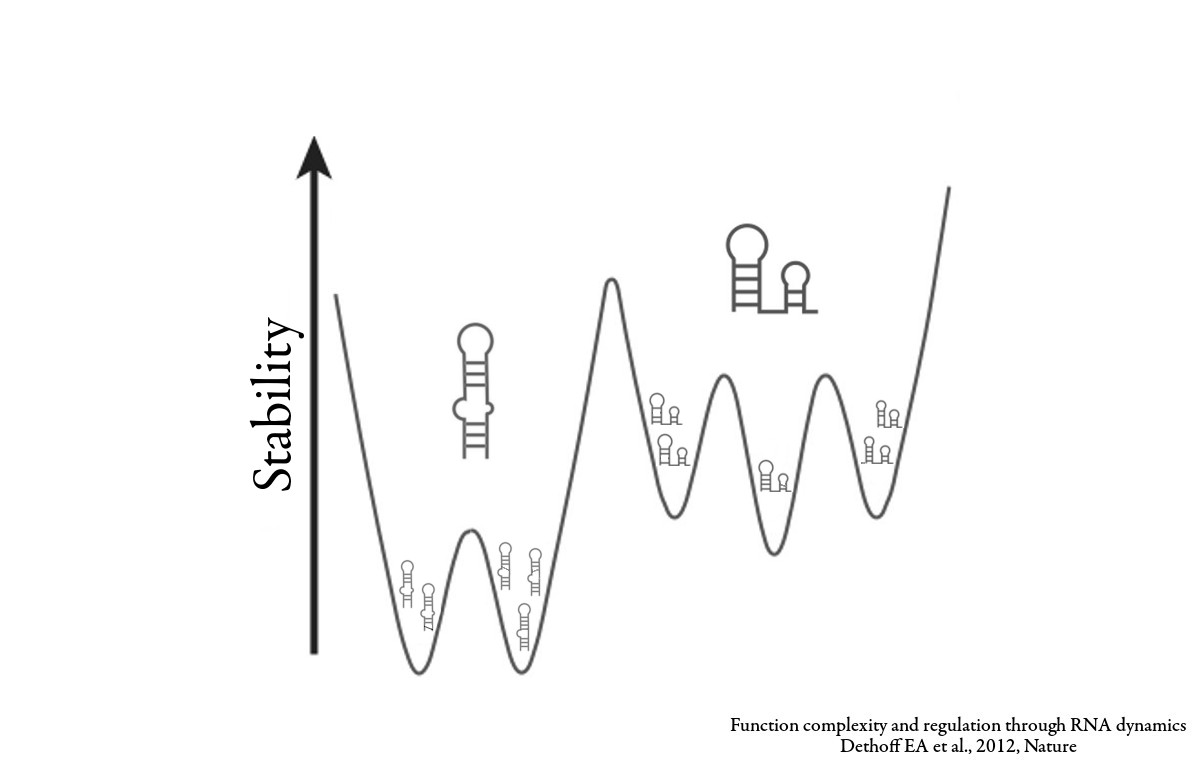
\includegraphics[scale=1.4]{figs/dynamics}
	%\caption{a single RNA molecule is present in many states}
	\end{figure}
\end{frame}


\begin{frame}
	\frametitle{softwares predict structure}

	\begin{itemize}
		\item MC-Fold (Parisien, Major, Nature, 2008)
		\item Mfold (Zuker, NAR, 2003)
		\item many others
	\end{itemize}
\end{frame}


\begin{frame}
	\frametitle{RNA families}
	\begin{figure}
	\centering
	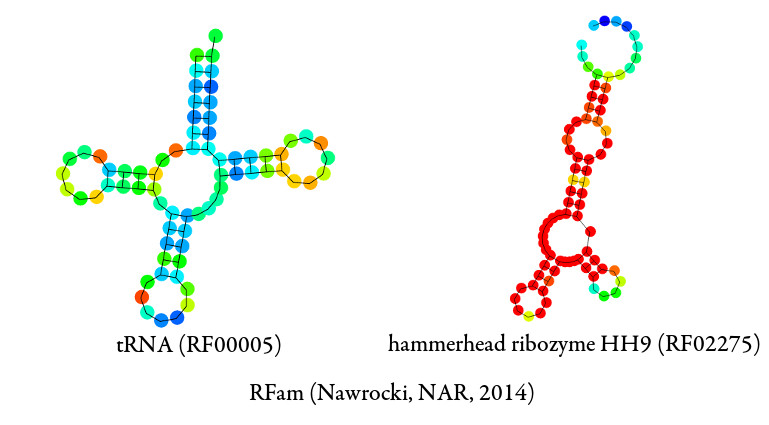
\includegraphics[scale=0.43]{figs/rfam}
	%\caption{many good potential structures}
	\end{figure}
\end{frame}


\begin{frame}

	\frametitle{what has been done}
	
	\begin{itemize}
		\item MC-Cons (Parisien, Major, Nature 2008)
		\item uses fold then align strategy (Gardner, Giegerich, BMC Bioinfo, 2003)
		\item good only for small and similar structures
	\end{itemize}
\end{frame}






\section{MC-Cons 2.0}

\begin{frame}
	\frametitle{RNA consensus}
	\begin{figure}
	\centering
	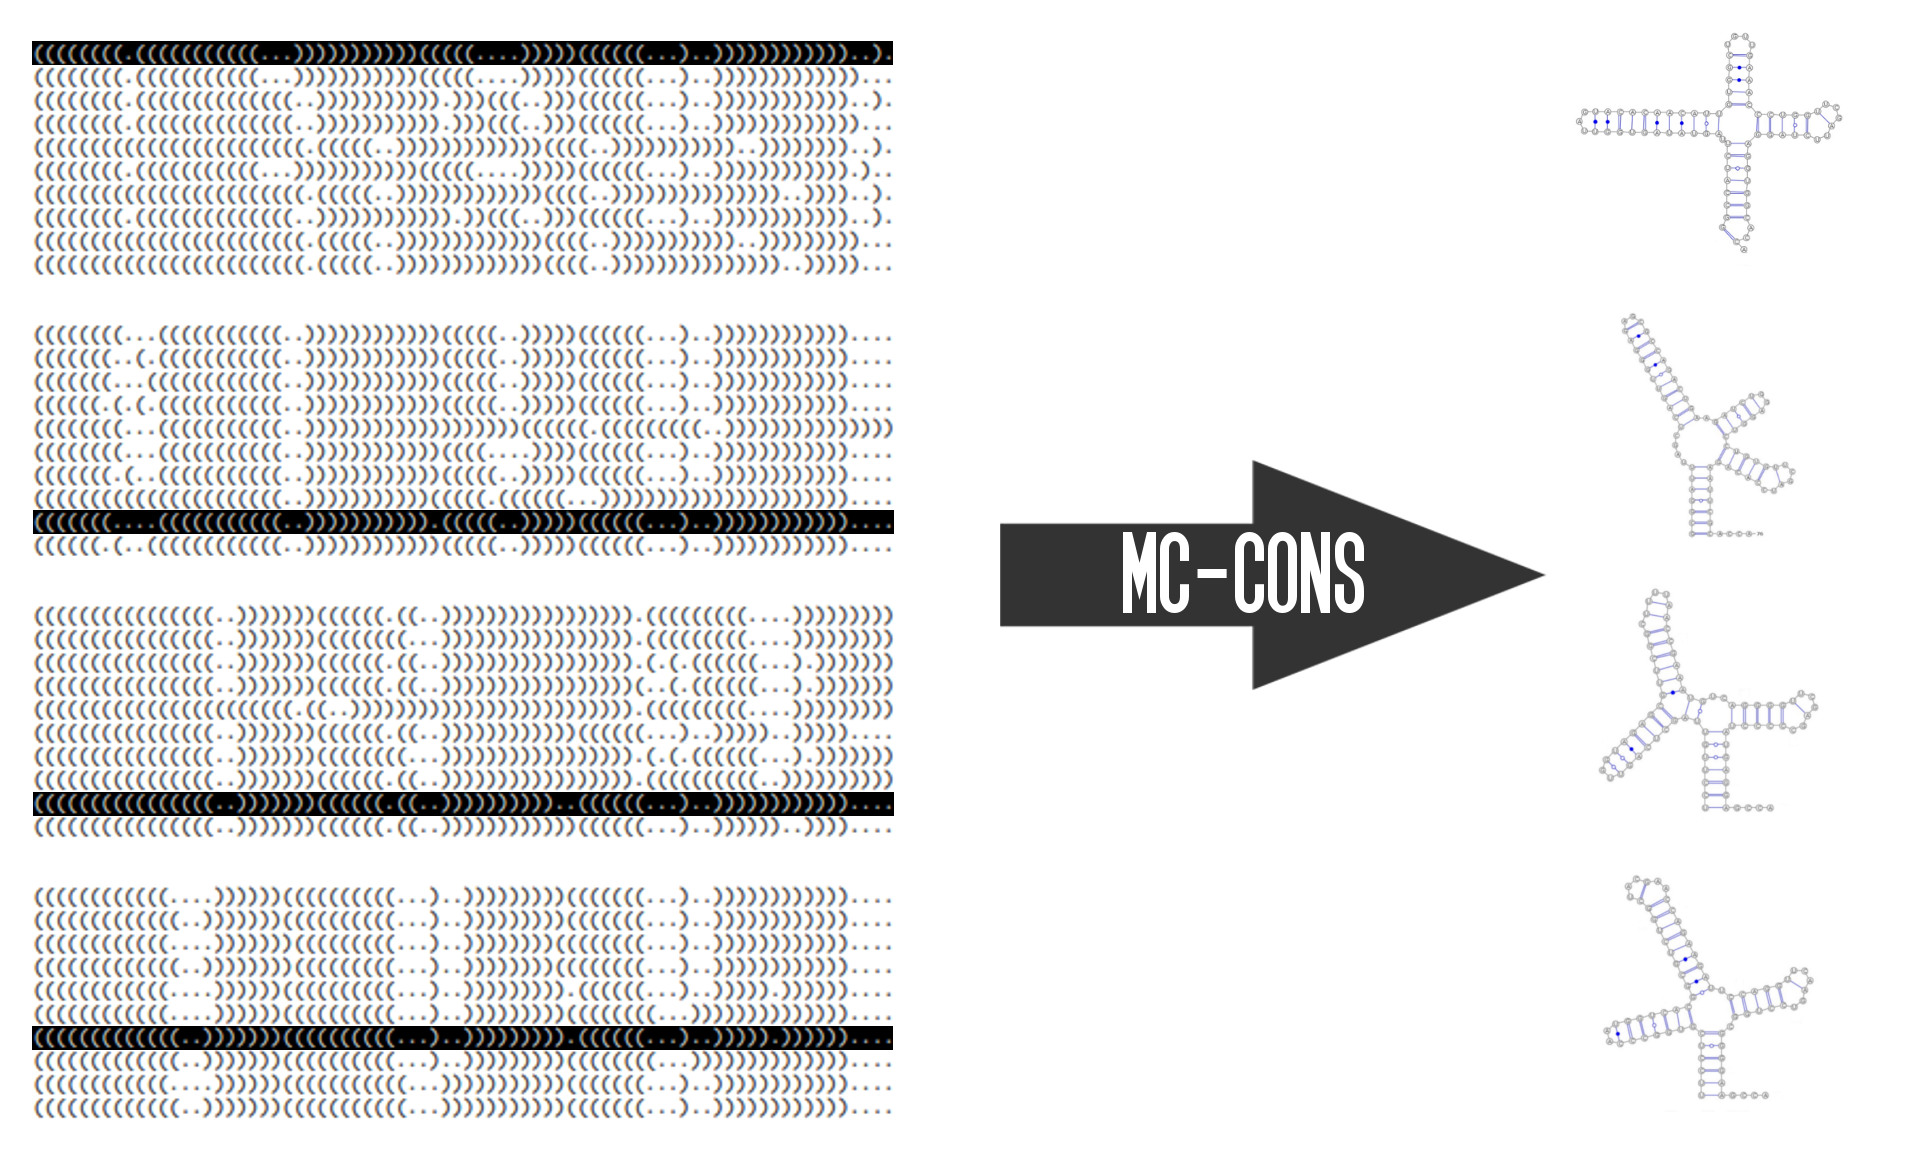
\includegraphics[scale=0.81]{figs/problem_setting}
	%\caption{}
	\end{figure}
\end{frame}




\begin{frame}
	\frametitle{computational approach}

	\begin{figure}
		\centering
		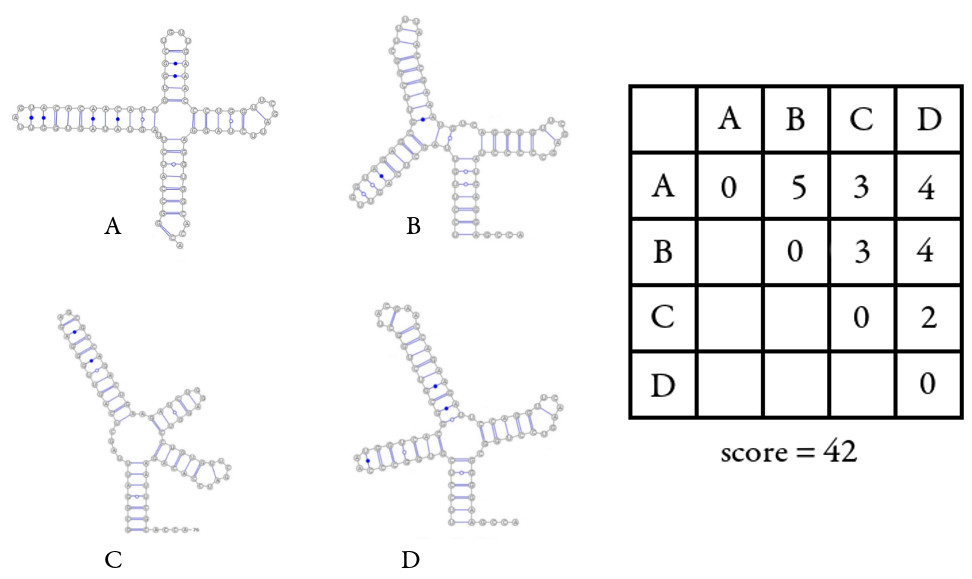
\includegraphics[scale=1.6]{figs/consensus}
	\end{figure}
	
%	\begin{itemize}
%		\item find pertinent distance function(s)		
%		\item minimize the sum of pairwise distances
%	\end{itemize}

\end{frame}



\begin{frame}
	\frametitle{it is very hard!}

	\begin{figure}
	\centering
	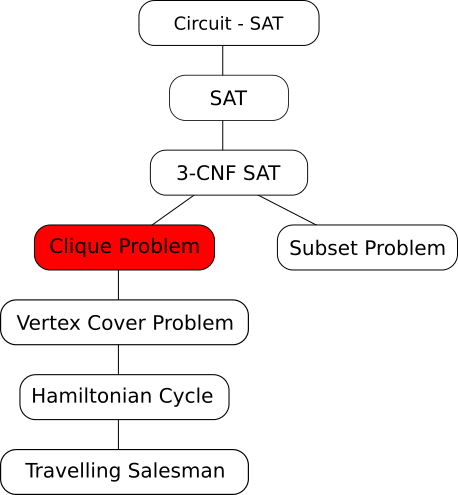
\includegraphics[scale=0.3]{figs/Relative_NPC_chart}
	%\caption{}
	\end{figure}
	\begin{itemize}
		\item result is the solution to max-clique
		\item exponential growth on input size
	\end{itemize}
	
\end{frame}


\begin{frame}
	\frametitle{heuristic approach}
		\begin{figure}
	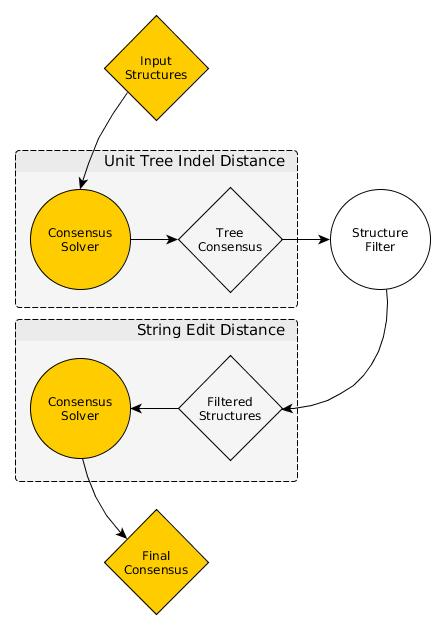
\includegraphics[scale=0.23]{figs/workflow}
	%\caption{}
	\end{figure}
	\begin{itemize}
		\item genetic algorithm (Barricelli, Methodos, 1954)
		\item local search
	\end{itemize}
	
\end{frame}


\section{results}

\begin{frame}
	\frametitle{Iron Response Elements}
	\begin{figure}
	\centering
	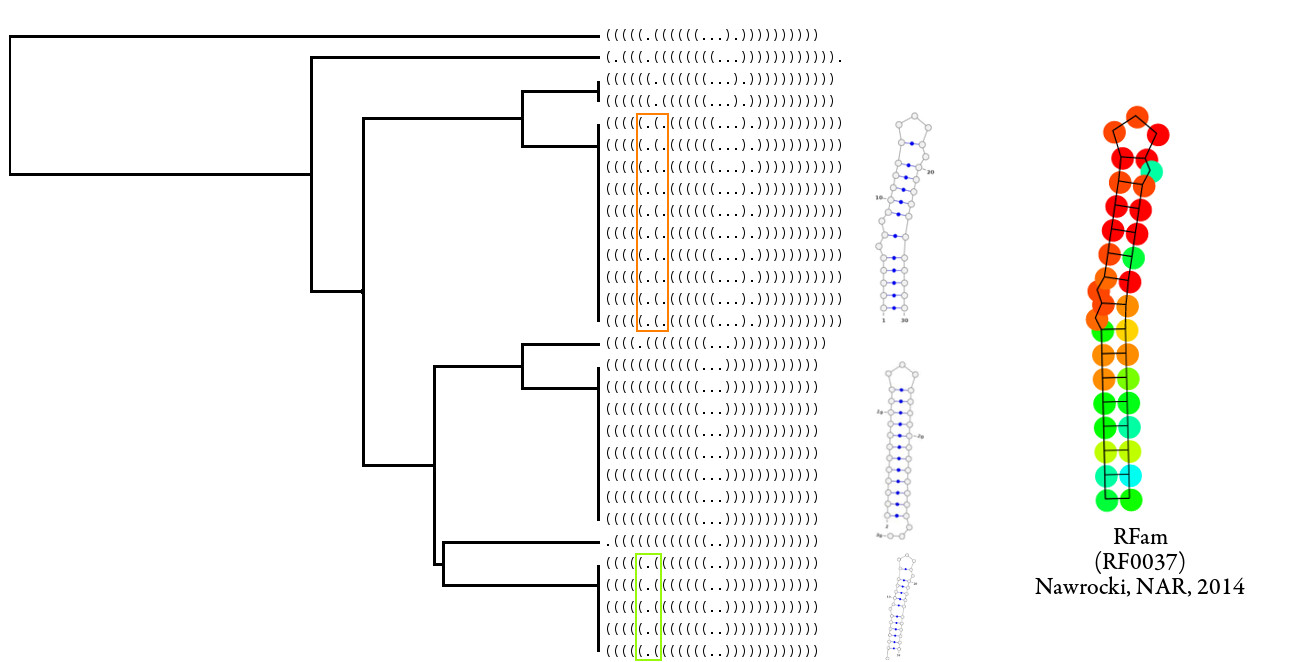
\includegraphics[scale=0.25]{figs/iresCons}
	%\caption{sometimes it works well!}
	\end{figure}
	
\end{frame}



\begin{frame}
	\frametitle{microRNAs}
	\begin{figure}
	\centering
	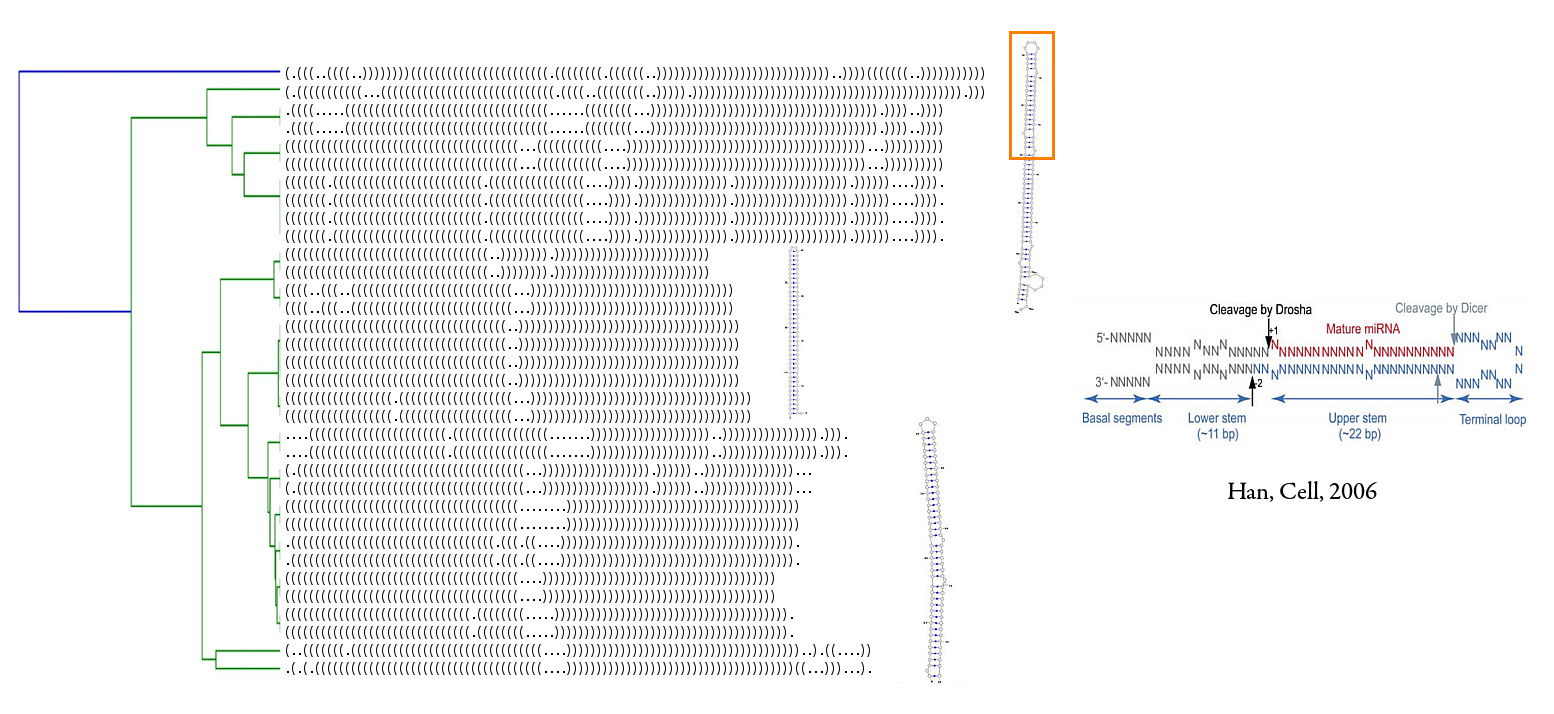
\includegraphics[scale=0.21]{figs/miRNACons}
	%\caption{}
	\end{figure}
	
\end{frame}


\section{conclusion}


% take home message
\begin{frame}
	\frametitle{summary}
	
	\begin{itemize}
		\item MC-Cons was slow, now its fast enough.
		\item Useful for exploration of RNA families with computational tools.
		\item It is easily extensible.
		\item Still some tweaking to do with the workflow.
	\end{itemize}

\end{frame}

\begin{frame}
	\frametitle{future work}
	\begin{itemize}
		\item Devise and implement better distance functions
		\item Multi-objective optimization to explore those distance functions (NSGA2)
		\item Implement relevance feedback to score consensus
		\end{itemize}
\end{frame}


\begin{frame}
	\frametitle{questions}
	\begin{figure}
	\centering
	
\includegraphics[scale=1]{figs/beer}
	%\caption{}
	\end{figure}
	
\end{frame}


% TODO add slide for distance functions




%\begin{frame}
%	\frametitle{now you can have consensus!}
%	\begin{figure}[!htb]
%	\centering
%	\resizebox{0.75\textwidth}{!}{\input{consensus_example.pdf_tex}}
%	\caption{Let's suppose that their function is explained by a subset of similar structures (consensus). \\\hspace{\textwidth}In this case, 2 consensus make sense. Sometimes you get more, sometimes you get less.}
%	\end{figure} 
%\end{frame}

%
%
%\section{why?}
%
%\begin{frame}
%	\frametitle{what's the point?}
%\begin{figure}[!htb]
%\centering
%\resizebox{0.55\textwidth}{!}{\input{consensus_banner.pdf_tex}}
%\end{figure} 
%
%	\begin{itemize}
%		
%		\item goal: finding common/similar structures within suboptimal secondary structures
%		\item useful for
%		\begin{itemize}
%			\item improving secondary structure prediction for functionally related RNAs
%			\item exploring shared alternative structures
%		\end{itemize}
%	\end{itemize}
%	
%\end{frame}
%
%
%\section{how?}
%
%\subsection{general workflow}
%\begin{frame}
%	\frametitle{workflow}
%	\begin{columns}
%		\column{0.38\linewidth}
%		\centering
%		\begin{figure}[!htb]
%			\resizebox{1.\textwidth}{!}{\input{workflow.pdf_tex}}
%		\end{figure} 
%        
%        \column{0.58\linewidth}
%        \begin{itemize}
%        		\item a consensus minimizes the sum of pairs of distances between objects
%        		\item optimization steps
%        		\begin{enumerate}
%        		        			\item base pair structural similarity (modified tree edit distance)
%        			\item string edit distance on Vienna dot-bracket representation
%        		\end{enumerate}
%			\item two solver in C++ (branch \& bound and genetic algorithm)
%        \end{itemize}
%         \end{columns}
%         
%\end{frame} 
%
%
%\subsection{matching base pairs}
%\begin{frame}
%	\frametitle{first match base pairs}
%	\begin{figure}[!htb]
%	\centering
%	\resizebox{0.4\textwidth}{!}{\input{bp_tree.pdf_tex}}
%	\end{figure} 
%	
%	\begin{itemize}
%		\item base pair trees created (many-to-one function)
%		\item unit tree indel distance calculates number of base pairs to add or remove to transform a tree into another
%	\end{itemize}
%	
%
%\end{frame}
%
%
%
%\subsection{match the bulges}
%\begin{frame}
%	\frametitle{then match unpaired}
%	\begin{figure}[!htb]
%	\centering
%	\resizebox{0.75\textwidth}{!}{\input{tree_filtering.pdf_tex}}
%	\end{figure}	
%	\begin{itemize}
%		\item filtered by tree structure, now refine
%		\item placing the bulges around the skeleton...
%		\item string edit distance on dot-bracket
%	\end{itemize}
%\end{frame}
%
%
%
%\section{examples}
%\subsection{IREs}
%\begin{frame}
%	\frametitle{IREs}
%	\begin{figure}[!htb]
%	\centering
%	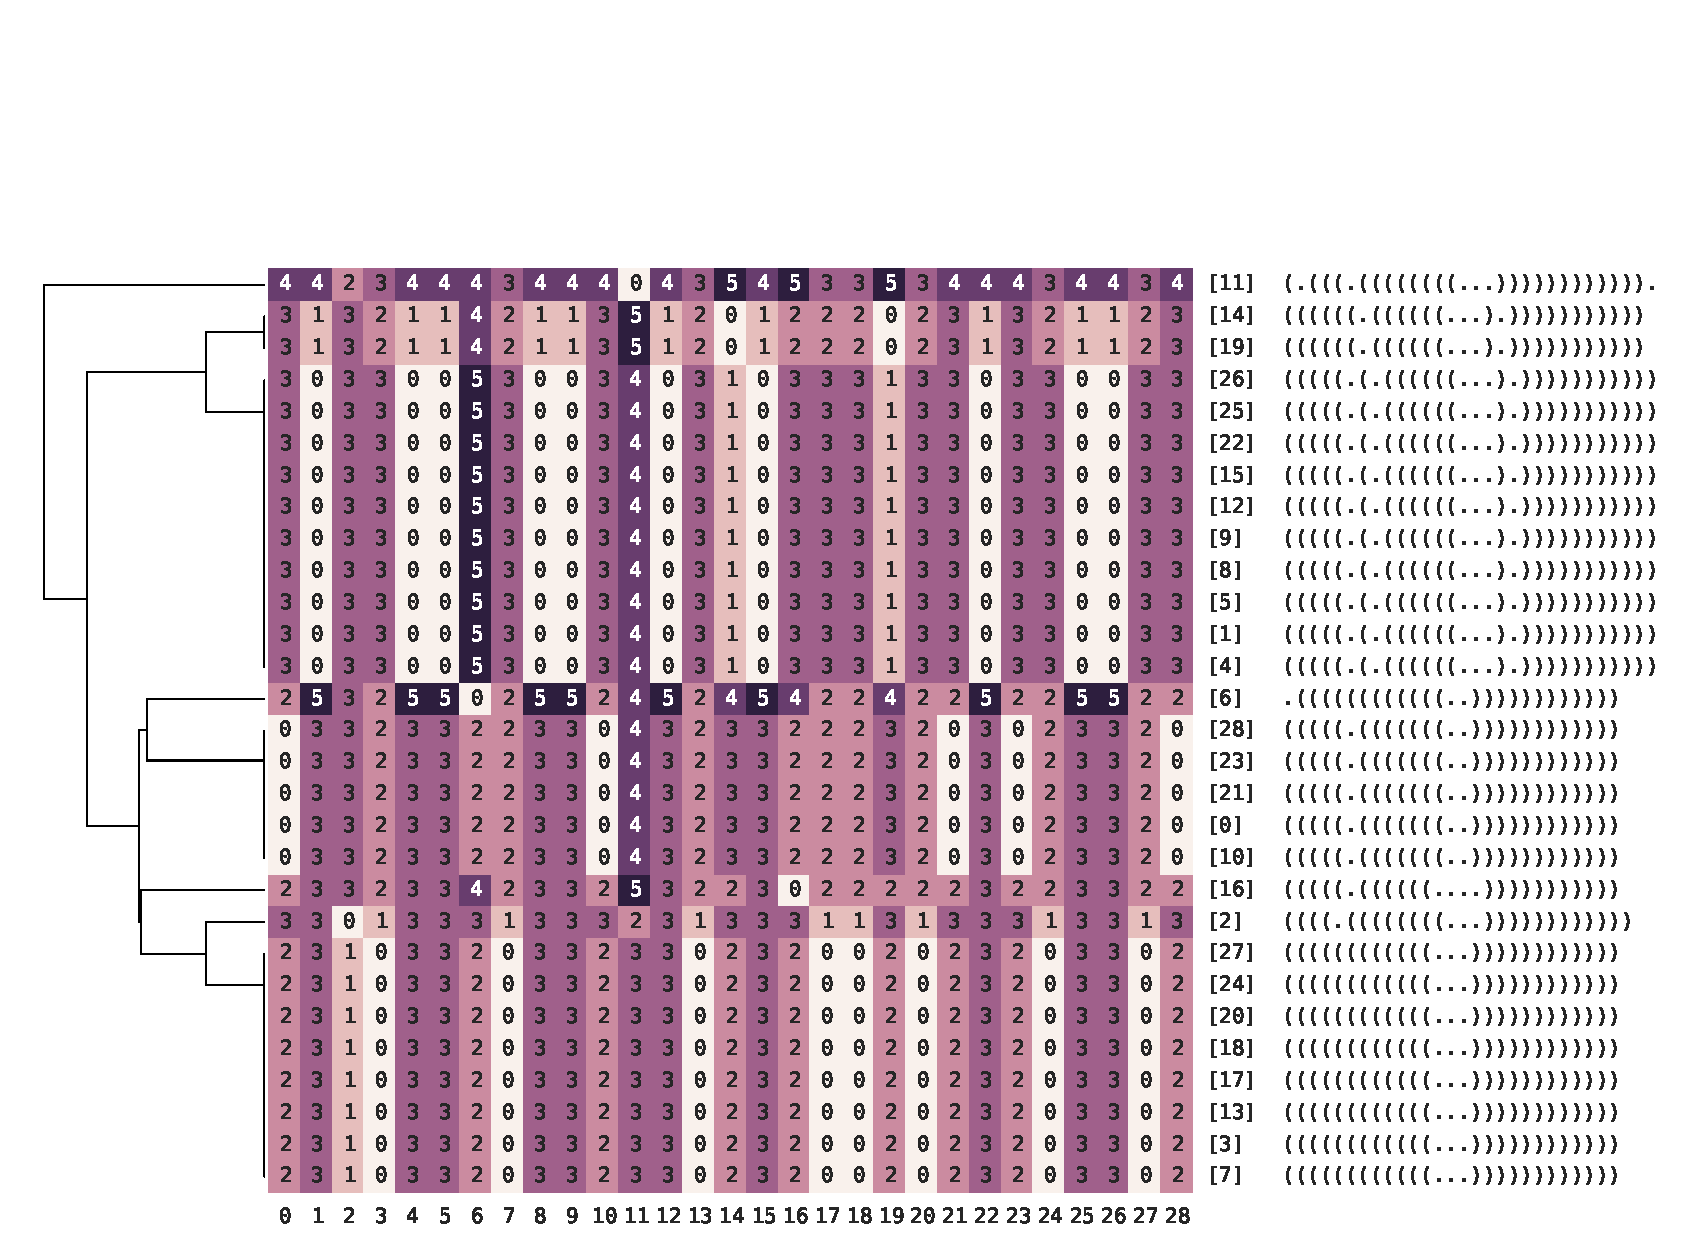
\includegraphics[scale=0.25]{figs/ires10.eps}
%	\caption{IREs structural assignment given 50 suboptimal for 29 different IREs.}
%	\end{figure} 
%\end{frame}
%
%
%
%\subsection{tRNAs}
%\begin{frame}
%	\frametitle{tRNAs}
%	
%
%\end{frame}
%
%

%
%
%
%\section{recap}
%
%\begin{frame}
%	\frametitle{recap}
%	\begin{itemize}
%		\item MC-Cons creates RNA 2D structural assignment
%		\item useful for finding structures explaining function
%		\item available at \url{https://github.com/major-lab/MC-Cons}
%	\end{itemize}
%\end{frame}
%
%\section{Q\&A}
%
%\begin{frame}
%	\frametitle{Q\&A}
%		\url{https://github.com/major-lab/MC-Cons}
%\end{frame}




\end{document}